% ======================================================================
% RAPPORT DE PROJET — DATA MINING (Master 2 IG/ID — ENEAM/UAC)
% Moteur : XeLaTeX via tectonic  ->  tectonic rapport_projet.tex
% Inspiré du style du cours « Data Warehouse » (boîtes pédagogiques tcolorbox).
% ======================================================================
\documentclass[11pt,a4paper]{article}

% ----- À COMPLÉTER ----------------------------------------------------
\newcommand{\professeur}{\textit{[Nom du professeur à compléter]}}
% (le corps du sujet PDF ne mentionne pas explicitement le nom ;
%  les métadonnées du fichier indiquent seulement « THED ».)
% ---------------------------------------------------------------------

\usepackage{fontspec}
\defaultfontfeatures{Ligatures=TeX}
\usepackage{polyglossia}
\setdefaultlanguage{french}
\providecommand{\og}{«\,}
\providecommand{\fg}{\,»}

\usepackage{geometry}
\geometry{left=2.4cm,right=2.4cm,top=2.5cm,bottom=2.5cm}

\usepackage{amsmath,amssymb}
\usepackage[table]{xcolor}
\usepackage{graphicx}
\usepackage{tikz}
\usetikzlibrary{calc, shapes.geometric, shapes.symbols, arrows.meta, positioning, fit, backgrounds}
\usepackage{hyperref}
\hypersetup{colorlinks=true, linkcolor=blue!55!black, urlcolor=blue!55!black}
\usepackage{enumitem}
\usepackage{tcolorbox}
\tcbuselibrary{skins, breakable}
\usepackage{listings}
\usepackage{array}
\usepackage{booktabs}
\usepackage{longtable}
\usepackage{titlesec}
\usepackage{fancyhdr}

% --- Couleurs ---
\definecolor{dmblue}{HTML}{1F4E79}
\definecolor{dmorange}{HTML}{C55A11}
\definecolor{dmgreen}{HTML}{385723}
\definecolor{dmgray}{HTML}{595959}
\definecolor{dmlight}{HTML}{F5F5F5}
\definecolor{codekw}{HTML}{0000AA}
\definecolor{codestr}{HTML}{AA0000}
\definecolor{codecom}{HTML}{008800}

% --- Couleurs page de garde (modèle TP1 Orion) ---
\definecolor{cBlue}{HTML}{1F4E79}      % bleu titres
\definecolor{cBlueBox}{HTML}{4472C4}   % bleu encadré titre page de garde
\definecolor{cBlueDeep}{HTML}{2E5C9E}  % bleu profond accent
\definecolor{cAccent}{HTML}{C8702A}    % orange accent décoratif

% --- Cadre décoratif de la page de garde ---
\newcommand{\drawCoverFrame}{%
  \begin{tikzpicture}[remember picture,overlay]
    \draw[cBlueBox, line width=2.2pt]
      ($(current page.north west)+(0.85cm,-0.85cm)$)
      rectangle ($(current page.south east)+(-0.85cm,0.85cm)$);
    \draw[cBlueBox, line width=0.45pt]
      ($(current page.north west)+(1.0cm,-1.0cm)$)
      rectangle ($(current page.south east)+(-1.0cm,1.0cm)$);
    \foreach \pos/\xs/\ys in {%
      north west/0.92cm/-0.92cm,
      north east/-0.92cm/-0.92cm,
      south west/0.92cm/0.92cm,
      south east/-0.92cm/0.92cm}{%
      \begin{scope}[shift={([shift={(\xs,\ys)}]current page.\pos)}]
        \node[diamond, fill=cBlueBox, draw=none,
              inner sep=0pt, minimum size=9mm] {};
        \node[diamond, fill=white, draw=cBlueBox, line width=0.4pt,
              inner sep=0pt, minimum size=6mm] {};
        \node[diamond, fill=cBlueDeep, draw=none,
              inner sep=0pt, minimum size=2.6mm] {};
        \fill[cAccent] (0,0) circle (0.5mm);
      \end{scope}
    }
  \end{tikzpicture}%
}

% --- En-tête / pied de page ---
\pagestyle{fancy}
\fancyhf{}
\fancyhead[L]{\small\color{dmgray}Projet Data Mining --- Master 2 IG/ID}
\fancyhead[R]{\small\color{dmgray}\thepage}
\renewcommand{\headrulewidth}{0.4pt}
\renewcommand{\headrule}{\hbox to\headwidth{\color{dmgray}\leaders\hrule height \headrulewidth\hfill}}

% --- Titres ---
\titleformat{\section}{\Large\bfseries\color{dmblue}}{\thesection}{1em}{}
\titleformat{\subsection}{\large\bfseries\color{dmorange}}{\thesubsection}{1em}{}
\titleformat{\subsubsection}{\normalsize\bfseries\color{dmgreen}}{\thesubsubsection}{1em}{}

% --- Boîtes pédagogiques ---
\newtcolorbox{definition}[1]{colback=dmblue!5, colframe=dmblue, fonttitle=\bfseries, title={#1}, breakable}
\newtcolorbox{exemple}[1][]{colback=dmorange!5, colframe=dmorange, fonttitle=\bfseries, title={Exemple #1}, breakable}
\newtcolorbox{regle}[1]{colback=dmgreen!5, colframe=dmgreen, fonttitle=\bfseries, title={#1}, breakable}
\newtcolorbox{attention}{colback=red!5, colframe=red!70!black, fonttitle=\bfseries, title=Attention, breakable}
\newtcolorbox{appbox}{colback=violet!4, colframe=violet!60!black, fonttitle=\bfseries, title=Le logiciel développé, breakable}

% --- Emplacement réservé pour une image (capture / figure WEKA) -------
% Usage : \captureph{légende explicative}{chemin/suggere.png}
\newcommand{\captureph}[2]{%
  \begin{center}
  \setlength{\fboxsep}{12pt}%
  \fcolorbox{dmblue}{dmlight}{%
    \begin{minipage}{0.86\textwidth}\centering
      {\color{dmblue}\large $\boxplus$\ \textbf{Emplacement image à insérer}}\\[5pt]
      {\small #1}\\[7pt]
      {\ttfamily\footnotesize\color{dmgray}\% \string\includegraphics[width=0.85\string\textwidth]\{\detokenize{#2}\}}\\[8pt]
      \rule{0pt}{3.2cm}%
    \end{minipage}}
  \end{center}}

% --- Code ---
\lstset{
  backgroundcolor=\color{dmlight},
  basicstyle=\ttfamily\footnotesize,
  keywordstyle=\color{codekw}\bfseries,
  stringstyle=\color{codestr},
  commentstyle=\color{codecom}\itshape,
  numbers=left, numberstyle=\tiny\color{dmgray}, numbersep=8pt,
  frame=single, rulecolor=\color{dmgray},
  breaklines=true, breakatwhitespace=true, showstringspaces=false,
  tabsize=2, captionpos=b,
  literate=%
    {é}{{\'e}}1 {è}{{\`e}}1 {ê}{{\^e}}1 {ë}{{\"e}}1
    {à}{{\`a}}1 {â}{{\^a}}1 {ô}{{\^o}}1 {î}{{\^i}}1 {û}{{\^u}}1
    {ù}{{\`u}}1 {ç}{{\c{c}}}1 {É}{{\'E}}1 {’}{{'}}1
}

\begin{document}

% ===================== PAGE DE GARDE (modèle TP1 Orion) ===============
\begin{titlepage}
\drawCoverFrame
\thispagestyle{empty}

\newcommand{\stars}[1]{{\bfseries\Large #1}}
\newcommand{\dualLine}[2]{{\bfseries #1\\[4pt]#2}}

\begin{tikzpicture}[remember picture, overlay]
  \node[anchor=north west, inner sep=0pt]
    at ([shift={(1.55cm,-1.55cm)}]current page.north west)
    {
\includegraphics[height=2.5cm]{images/logo-uac.png}};
  \node[anchor=north east, inner sep=0pt]
    at ([shift={(-1.55cm,-1.55cm)}]current page.north east)
    {
\includegraphics[height=2.5cm]{images/logo-eneam.jpg}};
\end{tikzpicture}%

\vspace*{0.05cm}
\begin{center}
  {\bfseries RÉPUBLIQUE DU BÉNIN}\\[7pt]
  \stars{********}\\[14pt]
  \dualLine{MINISTÈRE DE L'ENSEIGNEMENT SUPÉRIEUR ET DE LA}{RECHERCHE SCIENTIFIQUE (MESRS)}\\[7pt]
  \stars{*****************}\\[14pt]
  {\bfseries UNIVERSITÉ D'ABOMEY-CALAVI (UAC)}\\[7pt]
  \stars{**********}\\[14pt]
  {\bfseries ÉCOLE NATIONALE D'ÉCONOMIE APPLIQUÉE ET DE MANAGEMENT (ENEAM)}\\[7pt]
  \stars{******************}\\[14pt]
  {\bfseries DÉPARTEMENT INFORMATIQUE DE GESTION}\\[7pt]
  \stars{***********}\\[14pt]
  {\bfseries OPTION : INFORMATIQUE DÉCISIONNELLE}\\[7pt]
  \stars{***********}
\end{center}

\vspace{0.9cm}

\noindent\begin{minipage}[t]{0.5\textwidth}
  \textbf{Cycle} : Master
\end{minipage}\hfill
\begin{minipage}[t]{0.5\textwidth}\raggedleft
  \textbf{Matière} : Data Mining -- Fouille de données
\end{minipage}

\vspace{0.7cm}

\begin{center}
\begin{tcolorbox}[
  enhanced,
  colback=white, colframe=cBlueBox,
  boxrule=1.4pt, sharp corners,
  drop fuzzy shadow={cBlueBox!40},
  borderline={0.4pt}{4pt}{cBlueDeep,dashed},
  width=0.94\textwidth, halign=center, valign=center,
  left=22pt,right=22pt,top=18pt,bottom=14pt,
  overlay={%
    \foreach \pos in {north west, north east, south west, south east}{%
      \node[circle, draw=cBlueBox, line width=1.3pt, fill=white,
            inner sep=0pt, minimum size=15pt] (e\pos) at (frame.\pos) {};
      \fill[cBlueDeep] (e\pos.center) circle (1.6pt);
      \draw[cBlueBox, line width=0.5pt] (e\pos.center) circle (4pt);
    }
  }
]
  {\bfseries\normalsize\color{black} Rapport de projet :}\\[12pt]
  {\bfseries\Large\color{cBlue} DATA MINING : SEGMENTATION, CLASSIFICATION ET RECHERCHE D'ASSOCIATIONS}\\[6pt]
  {\bfseries\large\color{cBlueDeep} Conception d'une application et comparaison avec WEKA}
\end{tcolorbox}
\end{center}

\vspace{0.9cm}

\noindent\begin{minipage}[t]{0.55\textwidth}
  \textbf{Membres du groupe :}\\[8pt]
  \begin{enumerate}[leftmargin=*,topsep=0pt,itemsep=5pt]
    \item AKPO Amour
    \item GANDIGBE Ahowanou Gildas E.
  \end{enumerate}
\end{minipage}\hfill
\begin{minipage}[t]{0.42\textwidth}\raggedleft
  \textbf{Supervisé par :}\\[8pt]
  \professeur\\[4pt]
  \textbf{Enseignant à l'ENEAM}
\end{minipage}

\vfill

\begin{center}
\begin{tcolorbox}[
  colback=white, colframe=cBlueBox, boxrule=0.7pt, sharp corners,
  width=0.45\textwidth, halign=center,
  left=10pt,right=10pt,top=5pt,bottom=5pt
]
  \textbf{Année Académique} : 2025-2026
\end{tcolorbox}
\end{center}

\vspace*{0.2cm}
\end{titlepage}

\tableofcontents
\newpage

% ===================== 1. INTRODUCTION ================================
\section{Introduction et cahier des charges}

\subsection{Contexte}

Le \textbf{data mining} (fouille de données) regroupe les techniques permettant
d'extraire des connaissances utiles à partir de grands volumes de données. Trois
familles de tâches sont au cœur de ce projet :

\begin{itemize}[leftmargin=*]
  \item la \textbf{segmentation} (clustering) --- regrouper des individus qui se
        ressemblent, sans étiquette préalable (apprentissage \emph{non supervisé}) ;
  \item la \textbf{classification} --- prédire une classe connue à partir
        d'exemples étiquetés (apprentissage \emph{supervisé}) ;
  \item la \textbf{recherche d'associations} --- découvrir des règles
        \og si A alors B \fg{} dans des transactions.
\end{itemize}

\subsection{Travail à faire (rappel du sujet)}

\begin{regle}{Énoncé}
Concevoir une application graphique (Java ou Python) permettant d'exécuter les
\textbf{3 tâches} de data mining. L'application doit permettre de : (1) choisir la
tâche, (2) renseigner le chemin du dataset, (3) choisir l'algorithme, (4) lancer
l'analyse, (5) afficher les résultats, (6) utiliser un algorithme au choix par
tâche, (7) présenter les mesures de performance, (8) \textbf{comparer les
résultats à ceux de WEKA}.
\end{regle}

\subsection{Choix réalisés}

\begin{center}
\begin{tabular}{@{}p{3.6cm}p{4.6cm}p{5.4cm}@{}}
\toprule
\textbf{Tâche} & \textbf{Algorithme(s) implémenté(s)} & \textbf{Jeu de données utilisé} \\
\midrule
Segmentation & K-means & Credit Card (\texttt{cc\_general\_cluster.csv}) \\
Classification & Arbre de décision \& k-NN & Ionosphere (\texttt{Ionosphere\_classification.csv}) \\
Recherche d'associations & Apriori (\og maison \fg) & Wholesale customers (\texttt{wholesale\_association.csv}) \\
\bottomrule
\end{tabular}
\end{center}

\begin{exemple}[langage et outils]
L'application est écrite en \textbf{Python}. Les calculs reposent sur
\texttt{scikit-learn} (K-means, arbre, k-NN) et sur une implémentation
\textbf{personnelle} de l'algorithme Apriori. L'environnement est géré par
\texttt{uv} ; les analyses de référence sont rejouées dans \textbf{WEKA}.
\end{exemple}

% ===================== 2. ARCHITECTURE LOGICIELLE =====================
\section{Architecture de l'application}

\subsection{Une application, n'importe quel dataset}

\begin{appbox}
L'application \textbf{« Data Mining Studio »} (fichier \texttt{projet/app\_web.py},
interface web NiceGUI) implémente un \textbf{parcours guidé unique} valable pour
les trois tâches. Son principe directeur : \textbf{accepter n'importe quel fichier
CSV} fourni par l'utilisateur, puis adapter automatiquement les paramètres et
l'affichage à la tâche et à l'algorithme choisis.
\end{appbox}

\noindent Le parcours se déroule en six écrans :

\begin{center}
\begin{tikzpicture}[
  node distance=0.45cm and 0.55cm,
  etape/.style={rectangle, draw=dmblue, fill=dmblue!8, rounded corners,
               minimum height=1.05cm, minimum width=2.25cm, align=center, font=\scriptsize},
  arr/.style={-Stealth, thick, dmgray}]
\node[etape] (s1) {1. Tâche\\\scriptsize seg./classif./assoc.};
\node[etape, right=of s1] (s2) {2. Algorithme};
\node[etape, right=of s2] (s3) {3. Données\\\scriptsize upload CSV / démo};
\node[etape, right=of s3] (s4) {4. Paramètres};
\node[etape, right=of s4] (s5) {5. Calcul\\\scriptsize (thread)};
\node[etape, right=of s5] (s6) {6. Résultats\\\scriptsize métriques + graphes};
\draw[arr] (s1)--(s2); \draw[arr] (s2)--(s3); \draw[arr] (s3)--(s4);
\draw[arr] (s4)--(s5); \draw[arr] (s5)--(s6);
\end{tikzpicture}
\end{center}

\begin{itemize}[leftmargin=*]
  \item \textbf{Généricité de l'entrée.} L'écran 3 lit le CSV avec détection
        automatique du séparateur (\texttt{,} \texttt{;} ou tabulation) et affiche
        un aperçu paginé. Aucune colonne n'est codée en dur.
  \item \textbf{Adaptation à la tâche.} L'écran 4 propose les bons réglages :
        variable cible et taux de test (classification), nombre de clusters $K$ et
        normalisation (segmentation), colonne des paniers et seuils
        support/confiance (associations).
  \item \textbf{Calcul non bloquant.} L'analyse s'exécute dans un thread
        (\texttt{run.io\_bound}) pendant qu'un \emph{loader} tourne.
  \item \textbf{Restitution interactive.} L'écran 6 affiche les mesures de
        performance et des graphiques ECharts (matrice de confusion, projection
        des clusters, top des règles\ldots).
\end{itemize}

\subsection{Déclinaisons de l'interface}

Trois interfaces partagent le \textbf{même moteur de calcul} :

\begin{center}
\begin{tabular}{@{}p{3.2cm}p{4.1cm}p{6.0cm}@{}}
\toprule
\textbf{Fichier} & \textbf{Technologie} & \textbf{Usage} \\
\midrule
\texttt{app\_web.py} & NiceGUI (web) & version principale, thème sombre, ECharts \\
\texttt{app.py} & Streamlit & version tableau de bord rapide \\
\texttt{app\_tk.py} & Tkinter / customtkinter & version application de bureau \\
\bottomrule
\end{tabular}
\end{center}

\begin{lstlisting}[language=Python, caption={Cœur de calcul commun --- aiguillage par algorithme (\texttt{compute}, extrait simplifié)}]
def compute(cfg, df):
    algo = cfg["algo"]
    if algo in ("Arbre de décision", "k plus proches voisins"):
        X = pd.get_dummies(df[features]); y = df[cible].astype(str)
        Xtr, Xte, ytr, yte = train_test_split(X, y, test_size=cfg["split"],
                                              stratify=y, random_state=0)
        ...                       # arbre OU k-NN (avec standardisation)
    elif algo == "K-means":
        X = df.select_dtypes("number").to_numpy()
        if cfg["norm"]: X = StandardScaler().fit_transform(X)
        labels = KMeans(n_clusters=cfg["k"], n_init=10).fit_predict(X)
    elif algo == "Apriori":
        transactions = [set(str(v).split(",")) for v in df[cfg["col"]].dropna()]
        regles = regles_association(transactions, cfg["sup"], cfg["conf"])
\end{lstlisting}

\captureph{Capture de l'écran d'accueil de l'application (choix de la
tâche : Segmentation / Classification / Recherche d'associations).}
{figures/app_accueil.png}

% ===================== 3. SEGMENTATION ================================
\newpage
\section{Tâche 1 --- Segmentation (K-means)}

\subsection{Le logiciel pour cette tâche}

\begin{appbox}
Pour la segmentation, l'application sélectionne automatiquement
\textbf{toutes les colonnes numériques} du CSV chargé, propose une
\textbf{normalisation z-score} (activée par défaut), un curseur pour le
\textbf{nombre de clusters $K$}, puis affiche la \textbf{silhouette}, l'inertie,
la taille des clusters et une \textbf{projection 2D par ACP}. Le même écran
fonctionne pour Credit Card comme pour tout autre tableau numérique.
\end{appbox}

\subsection{Contexte du jeu de données : Credit Card}

\begin{definition}{Dataset Credit Card}
8\,950 titulaires de cartes de crédit décrits par \textbf{17 variables}
comportementales sur 6 mois (solde, achats, avances de trésorerie, fréquences,
limites, paiements\ldots). Aucune étiquette : l'objectif est de \textbf{découvrir
des profils de clients} pour le marketing.
\end{definition}

\noindent Variables principales : \texttt{BALANCE}, \texttt{PURCHASES},
\texttt{ONEOFF\_PURCHASES}, \texttt{INSTALLMENTS\_PURCHASES},
\texttt{CASH\_ADVANCE}, les fréquences associées (\texttt{*\_FREQUENCY}),
\texttt{CREDIT\_LIMIT}, \texttt{PAYMENTS}, \texttt{MINIMUM\_PAYMENTS},
\texttt{PRC\_FULL\_PAYMENT}, \texttt{TENURE}.

\subsection{Données AVANT prétraitement}

Extrait du fichier brut (\texttt{CC GENERAL.csv}) --- noter l'identifiant et une
valeur manquante :

\begin{center}\footnotesize
\begin{tabular}{@{}lrrrrrr@{}}
\toprule
\texttt{CUST\_ID} & \texttt{BALANCE} & \texttt{PURCHASES} & \texttt{CASH\_ADV.} & \texttt{CREDIT\_LIM.} & \texttt{MIN\_PAY.} & \texttt{TENURE} \\
\midrule
C10001 & 40.90 & 95.40 & 0.00 & 1000 & 139.51 & 12 \\
C10002 & 3202.47 & 0.00 & 6442.95 & 7000 & 1072.34 & 12 \\
C10003 & 2495.15 & 773.17 & 0.00 & 7500 & 627.28 & 12 \\
C10004 & 1666.67 & 1499.00 & 205.79 & 7500 & \cellcolor{red!12}\textit{(vide)} & 12 \\
\bottomrule
\end{tabular}
\end{center}

\begin{attention}
Trois problèmes rendent ces données \textbf{inexploitables telles quelles} par
K-means : (1) \texttt{CUST\_ID} n'est pas une mesure ; (2) des valeurs manquantes
(\texttt{MINIMUM\_PAYMENTS} $\approx$ 313 cas, \texttt{CREDIT\_LIMIT} 1 cas) ;
(3) des \textbf{échelles très hétérogènes} (montants en milliers vs fréquences
dans $[0,1]$) et des distributions \textbf{très asymétriques}.
\end{attention}

\subsection{Zoom sur le prétraitement appliqué}

\begin{regle}{Chaîne de prétraitement (script \texttt{scripts/cc\_preprocessing.py})}
\begin{enumerate}[leftmargin=*]
  \item \textbf{Retrait de \texttt{CUST\_ID}} : identifiant, fausserait les distances.
  \item \textbf{Imputation par la médiane} (\texttt{MINIMUM\_PAYMENTS},
        \texttt{CREDIT\_LIMIT}) : robuste à l'asymétrie.
  \item \textbf{Transformation log} ($\log(1+x)$) sur les variables monétaires :
        compresse les longues queues et symétrise les distributions.
  \item \textbf{Winsorisation 1\,\%/99\,\%} : borne les valeurs extrêmes
        \emph{sans supprimer} de clients.
  \item \textbf{Standardisation z-score} : étape critique --- K-means et l'ACP
        reposent sur la distance euclidienne ; sans elle, \texttt{BALANCE}
        écraserait les fréquences.
\end{enumerate}
\end{regle}

\noindent \textbf{Effet mesuré de la transformation log} sur l'asymétrie
(\emph{skewness}, proche de 0 = symétrique) :

\begin{center}\footnotesize
\begin{tabular}{@{}lrr@{}}
\toprule
\textbf{Variable} & \textbf{Skewness avant} & \textbf{Skewness après log} \\
\midrule
\texttt{PURCHASES} & 8.14 & $-0.76$ \\
\texttt{CASH\_ADVANCE} & 5.17 & 0.26 \\
\texttt{PAYMENTS} & 5.91 & $-1.78$ \\
\texttt{MINIMUM\_PAYMENTS} & 13.85 & 0.27 \\
\bottomrule
\end{tabular}
\end{center}

\begin{definition}{Standardisation (z-score)}
\[
x^\star = \frac{x - \overline{x}}{\sigma_x}
\]
Après transformation, chaque variable a une moyenne nulle et un écart-type de 1
(vérifié : moyenne $\approx 10^{-16}$, $\sigma \approx 1.00$).
\end{definition}

\subsection{Données APRÈS prétraitement}

Matrice de corrélation (après nettoyage) --- elle révèle les redondances, gérées
ensuite par l'ACP :

\begin{center}
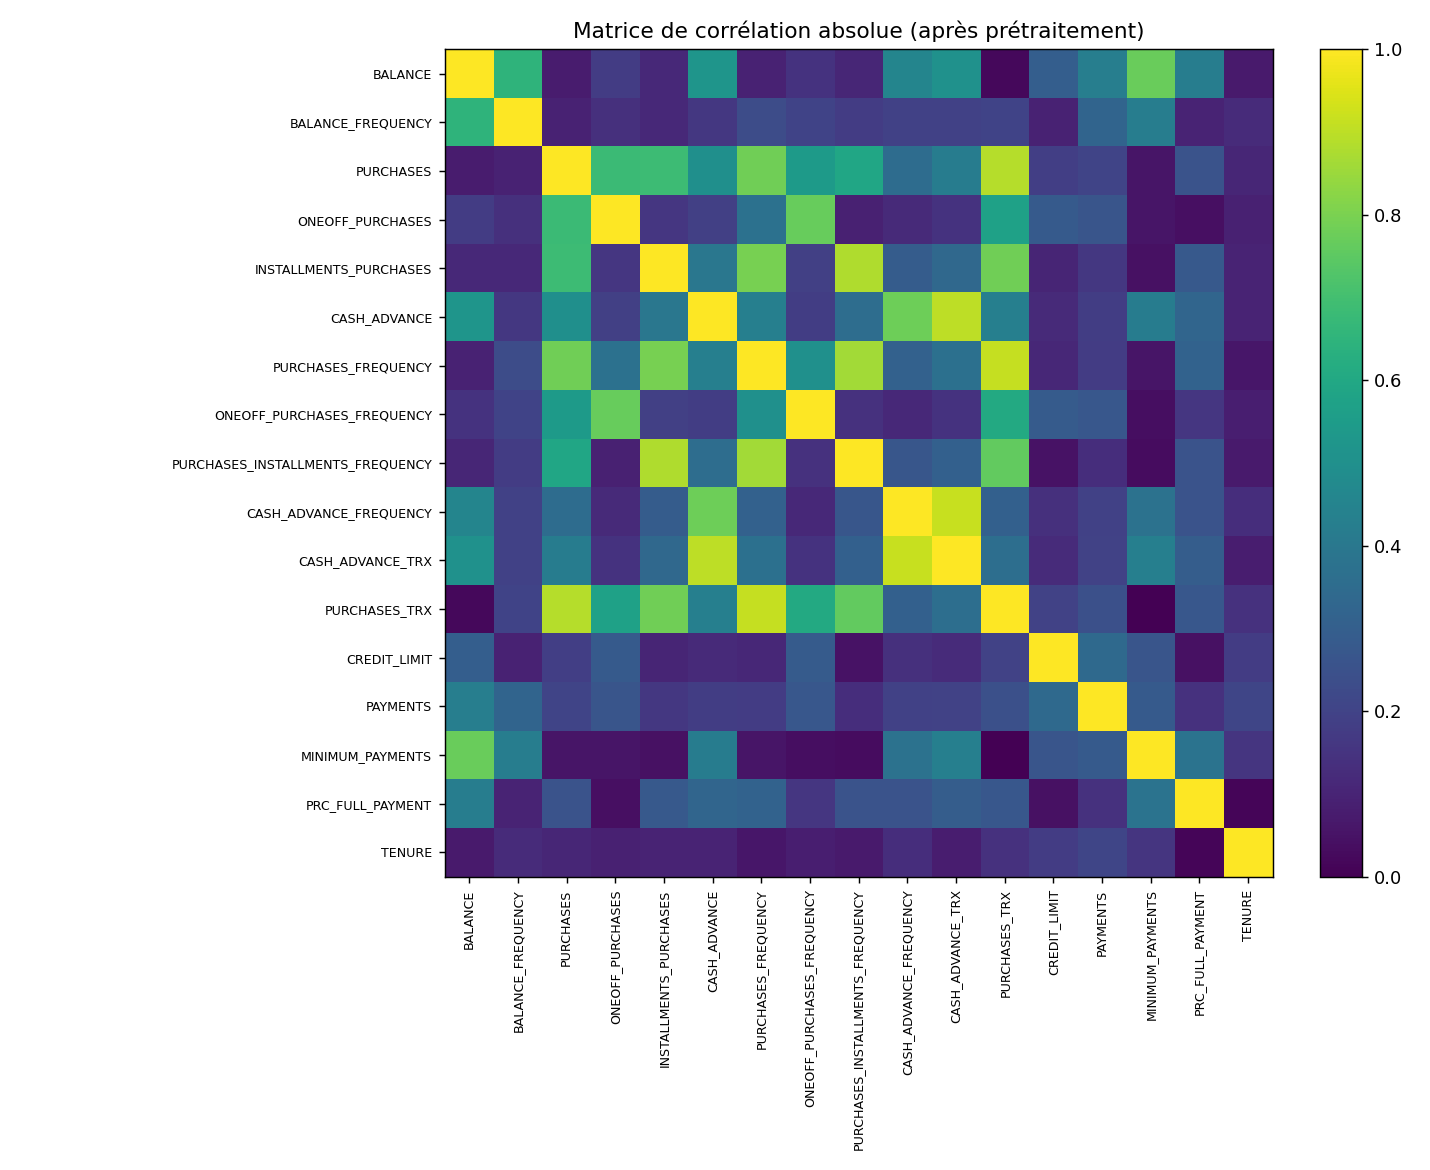
\includegraphics[width=0.62\textwidth]{figures/cc_correlation.png}
\end{center}

\subsection{Choix de $K$ et mesures de performance}

\begin{definition}{Mesures de qualité d'une partition}
\begin{itemize}[leftmargin=*]
  \item \textbf{Inertie intra-cluster} : somme des distances au centre ; on
        cherche le \og coude \fg{} de la courbe.
  \item \textbf{Silhouette} $\in [-1,1]$ : compare la cohésion interne à la
        séparation entre clusters ; plus elle est haute, mieux c'est.
\end{itemize}
\end{definition}

\begin{center}
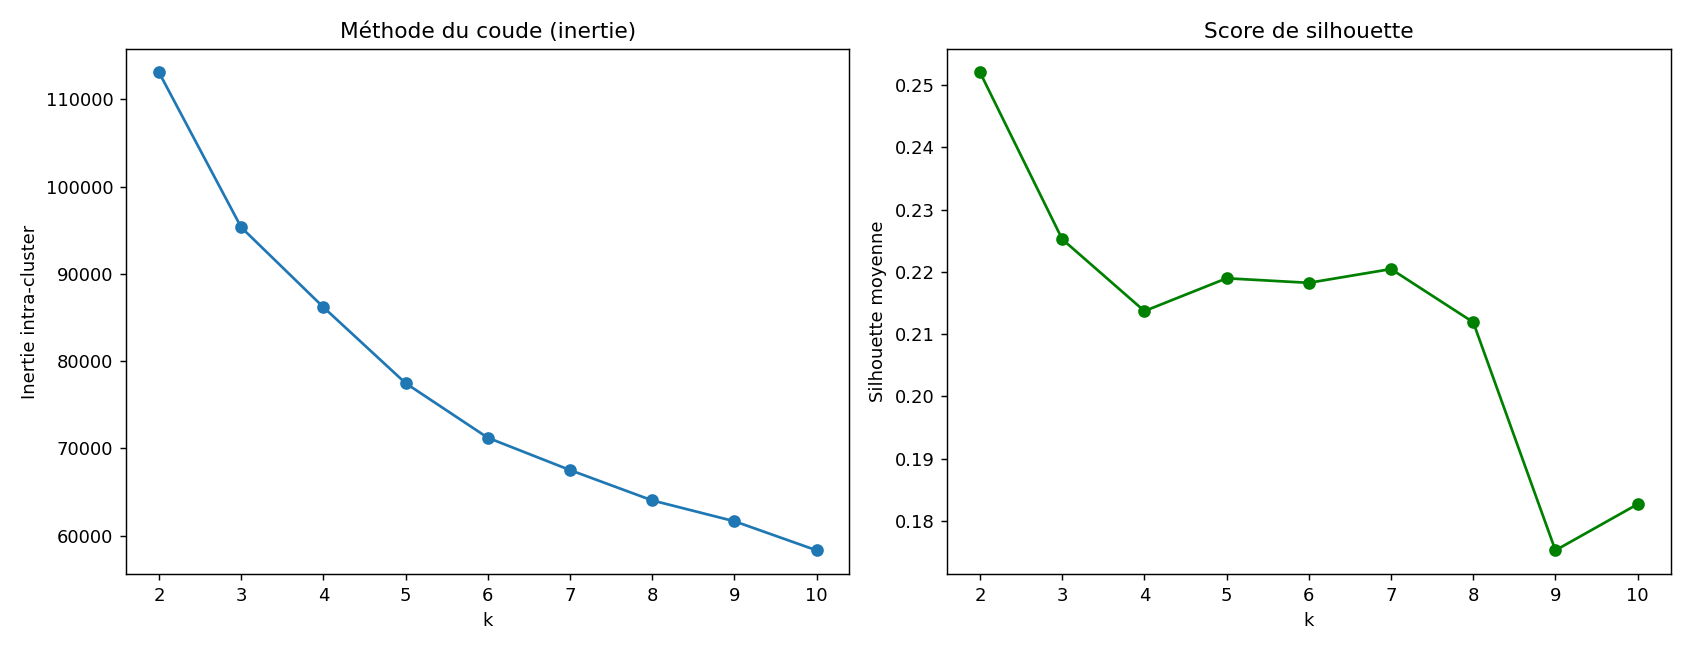
\includegraphics[width=0.92\textwidth]{figures/cc_choix_k.png}
\end{center}

\begin{exemple}[résultat obtenu]
La silhouette est maximale pour $K=2$ (silhouette $\approx 0.25$). La courbe du
coude suggère un second compromis vers $K=4$--$6$, plus fin pour le marketing.
\end{exemple}

\subsection{Résultats dans notre application}

\begin{center}
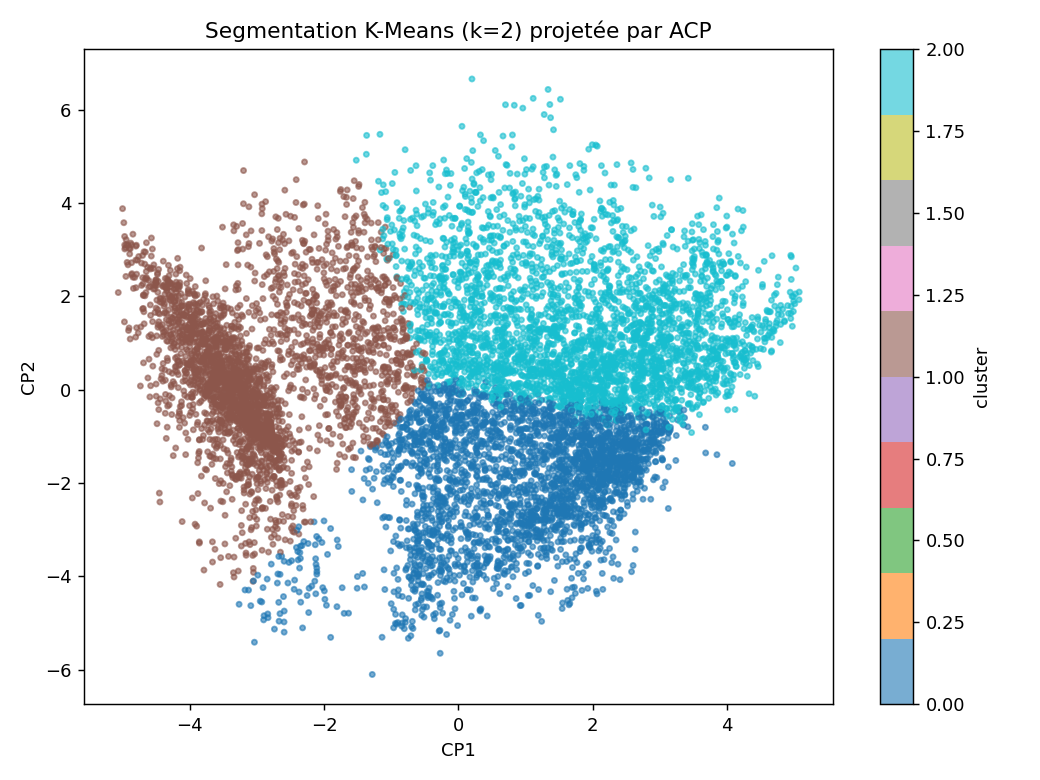
\includegraphics[width=0.66\textwidth]{figures/cc_clusters_acp.png}
\end{center}

\noindent Profils moyens (en unités réelles) des deux segments obtenus :

\begin{center}\footnotesize
\begin{tabular}{@{}lrr@{}}
\toprule
\textbf{Variable (moyenne)} & \textbf{Segment 0} & \textbf{Segment 1} \\
\midrule
Effectif & 5\,779 & 3\,171 \\
\texttt{PURCHASES} & 1\,471.9 & 149.0 \\
\texttt{CASH\_ADVANCE} & 335.9 & 2\,150.7 \\
\texttt{PURCHASES\_TRX} & 21.8 & 1.8 \\
\texttt{CASH\_ADVANCE\_TRX} & 1.1 & 7.1 \\
\midrule
\textbf{Interprétation} & \textit{Acheteurs} & \textit{Emprunteurs cash} \\
\bottomrule
\end{tabular}
\end{center}

\captureph{Capture de l'écran de résultats K-means dans l'application (cartes
silhouette / inertie / nombre de clusters et nuage de points coloré).}
{figures/app_kmeans_resultats.png}

\subsection{Résultats avec WEKA}

\begin{exemple}[mode opératoire WEKA]
Charger \texttt{cc\_general\_cluster.csv} (onglet \emph{Preprocess}, après
standardisation) $\rightarrow$ onglet \emph{Cluster} $\rightarrow$
\texttt{SimpleKMeans} $\rightarrow$ régler \texttt{numClusters} $\rightarrow$
\emph{Start}. Relever les centres et la somme des erreurs quadratiques.
\end{exemple}

\captureph{Capture WEKA --- résultat de \texttt{SimpleKMeans} (centres des
clusters et \emph{Within cluster sum of squared errors}).}
{figures/weka_kmeans.png}

\subsection{Comparaison application vs WEKA}

\begin{center}
\begin{tabular}{@{}p{4.2cm}p{4.3cm}p{4.3cm}@{}}
\toprule
\textbf{Critère} & \textbf{Notre application} & \textbf{WEKA (SimpleKMeans)} \\
\midrule
Nombre de clusters & \textit{(à reporter)} & \textit{(à reporter)} \\
Effectifs par cluster & \textit{(à reporter)} & \textit{(à reporter)} \\
Inertie / SSE & \textit{(à reporter)} & \textit{(à reporter)} \\
Interprétation des profils & \textit{(à reporter)} & \textit{(à reporter)} \\
\bottomrule
\end{tabular}
\end{center}

% ===================== 4. CLASSIFICATION ==============================
\newpage
\section{Tâche 2 --- Classification (Arbre de décision \& k-NN)}

\subsection{Le logiciel pour cette tâche}

\begin{appbox}
Pour la classification, l'utilisateur choisit la \textbf{variable cible} (par
défaut la dernière colonne) et le \textbf{taux de test}. Les variables
catégorielles sont automatiquement encodées (\texttt{get\_dummies}) ; pour le
k-NN, les variables sont \textbf{standardisées}. L'application affiche
l'\textbf{exactitude}, la \textbf{précision}, le \textbf{rappel}, le
\textbf{F1-score}, la \textbf{matrice de confusion} et, pour l'arbre, sa
\textbf{visualisation}. Tout CSV étiqueté est accepté.
\end{appbox}

\subsection{Contexte du jeu de données : Ionosphere}

\begin{definition}{Dataset Ionosphere}
351 relevés radar de l'ionosphère, décrits par \textbf{34 attributs numériques}
(parties réelle/imaginaire de 17 signaux) et une classe binaire
\texttt{Class} : \og good \fg{} (signal structuré, 225 cas) vs \og bad \fg{}
(126 cas). Tâche : \textbf{prédire} la qualité du retour radar.
\end{definition}

\subsection{Données AVANT / APRÈS prétraitement}

\begin{center}\footnotesize
\begin{tabular}{@{}lrrrrr@{}}
\toprule
& \texttt{V1} & \texttt{V2} & \texttt{V3} & \texttt{V34} & \texttt{Class} \\
\midrule
ex. 1 & 1 & 0 & 0.99539 & $-0.45300$ & 1 \\
ex. 2 & 1 & 0 & 1.00000 & $\ldots$ & 1 \\
\bottomrule
\end{tabular}
\end{center}

\begin{regle}{Prétraitement appliqué}
\begin{enumerate}[leftmargin=*]
  \item \textbf{Aucune valeur manquante} (vérifié) : pas d'imputation nécessaire.
  \item \textbf{Suppression de \texttt{V2}} : colonne \textbf{constante} (toujours
        0), donc variance nulle, sans pouvoir discriminant.
  \item \textbf{Variables déjà bornées} dans $[-1,1]$ : pour l'arbre, aucune mise
        à l'échelle n'est requise ; pour le \textbf{k-NN}, on applique le
        \textbf{z-score} (la distance euclidienne l'exige).
  \item \textbf{Découpage stratifié} apprentissage / test (préserve la proportion
        good/bad).
\end{enumerate}
\end{regle}

\captureph{Aperçu du dataset Ionosphere chargé dans l'application (table
paginée, écran « Données »).}{figures/app_ionosphere_apercu.png}

\subsection{Algorithmes et mesures de performance}

\begin{definition}{Métriques de classification}
À partir de la matrice de confusion (VP, FP, VN, FN) :
\[
\text{Exactitude}=\frac{VP+VN}{\text{total}},\quad
\text{Précision}=\frac{VP}{VP+FP},\quad
\text{Rappel}=\frac{VP}{VP+FN},
\]
\[
F_1 = 2\cdot\frac{\text{Précision}\cdot\text{Rappel}}{\text{Précision}+\text{Rappel}}.
\]
\end{definition}

\begin{itemize}[leftmargin=*]
  \item \textbf{Arbre de décision} : suite de tests oui/non sur les attributs
        (paramètre : profondeur maximale).
  \item \textbf{k plus proches voisins (k-NN)} : vote des $k$ voisins les plus
        proches (paramètre : $k$, données standardisées).
\end{itemize}

\subsection{Résultats dans notre application}

\begin{center}
\begin{tabular}{@{}lrrrr@{}}
\toprule
\textbf{Algorithme} & \textbf{Exactitude} & \textbf{Précision} & \textbf{Rappel} & \textbf{F1} \\
\midrule
Arbre de décision & \textit{(à reporter)} & \textit{(à reporter)} & \textit{(à reporter)} & \textit{(à reporter)} \\
k-NN & \textit{(à reporter)} & \textit{(à reporter)} & \textit{(à reporter)} & \textit{(à reporter)} \\
\bottomrule
\end{tabular}
\end{center}

\captureph{Capture des résultats de classification (cartes de métriques +
matrice de confusion ECharts).}{figures/app_classif_resultats.png}

\captureph{Capture de l'arbre de décision affiché par l'application
(\texttt{plot\_tree}, 3 premiers niveaux).}{figures/app_arbre.png}

\subsection{Résultats avec WEKA}

\begin{exemple}[mode opératoire WEKA]
Charger \texttt{Ionosphere\_classification.csv}, définir \texttt{Class} comme
attribut de classe, onglet \emph{Classify} : \texttt{trees $\rightarrow$ J48}
(équivalent de l'arbre) et \texttt{lazy $\rightarrow$ IBk} (équivalent du k-NN),
validation croisée 10 plis. Relever \emph{Correctly Classified Instances},
précision, rappel, F-measure et la \emph{Confusion Matrix}.
\end{exemple}

\captureph{Capture WEKA --- sortie de \texttt{J48} et/ou \texttt{IBk}
(récapitulatif des performances et matrice de confusion).}{figures/weka_classif.png}

\subsection{Comparaison application vs WEKA}

\begin{center}
\begin{tabular}{@{}p{3.2cm}rr@{\hskip 1.2em}rr@{}}
\toprule
& \multicolumn{2}{c}{\textbf{Notre application}} & \multicolumn{2}{c}{\textbf{WEKA}} \\
\cmidrule(lr){2-3}\cmidrule(lr){4-5}
\textbf{Métrique} & Arbre & k-NN & J48 & IBk \\
\midrule
Exactitude & \textit{...} & \textit{...} & \textit{...} & \textit{...} \\
Précision  & \textit{...} & \textit{...} & \textit{...} & \textit{...} \\
Rappel     & \textit{...} & \textit{...} & \textit{...} & \textit{...} \\
F1         & \textit{...} & \textit{...} & \textit{...} & \textit{...} \\
\bottomrule
\end{tabular}
\end{center}

% ===================== 5. ASSOCIATIONS ================================
\newpage
\section{Tâche 3 --- Recherche d'associations (Apriori)}

\subsection{Le logiciel pour cette tâche}

\begin{appbox}
L'application implémente Apriori \textbf{à la main} (\texttt{projet/apriori.py}).
L'utilisateur choisit la colonne des \textbf{paniers} (articles séparés par des
virgules) et règle le \textbf{support} et la \textbf{confiance} minimaux. Sont
affichés : le nombre de règles, un tableau \og Si\ldots Alors \fg{} avec support,
confiance et \textbf{lift}, et un graphique des meilleures règles.
\end{appbox}

\begin{definition}{Support, confiance, lift}
\[
\text{support}(X)=\frac{\#\{\text{transactions} \supseteq X\}}{N},\quad
\text{confiance}(X\!\to\!Y)=\frac{\text{support}(X\cup Y)}{\text{support}(X)},
\]
\[
\text{lift}(X\!\to\!Y)=\frac{\text{confiance}(X\!\to\!Y)}{\text{support}(Y)}
\quad (>1 : \text{corrélation positive}).
\]
\end{definition}

\subsection{Contexte du jeu de données : Wholesale customers}

\begin{definition}{Dataset Wholesale}
440 clients d'un grossiste, décrits par leurs \textbf{dépenses annuelles} dans 6
catégories : \texttt{Fresh}, \texttt{Milk}, \texttt{Grocery}, \texttt{Frozen},
\texttt{Detergents\_Paper}, \texttt{Delicassen}. But : trouver quelles catégories
sont \textbf{achetées ensemble} à des niveaux comparables.
\end{definition}

\subsection{Zoom sur le prétraitement : de montants à transactions}

\begin{attention}
Apriori travaille sur des \textbf{items discrets}, pas sur des montants continus.
Le dataset brut (dépenses en euros) doit donc être \textbf{discrétisé}.
\end{attention}

\begin{regle}{Prétraitement appliqué}
\begin{enumerate}[leftmargin=*]
  \item \textbf{Discrétisation} de chaque dépense en \textbf{5 niveaux} par
        quantiles : \texttt{Très faible}, \texttt{Faible}, \texttt{Moyen},
        \texttt{Fort}, \texttt{Très fort} (fichier \texttt{wholesale\_association.csv}).
  \item \textbf{Construction des transactions} : chaque ligne devient un panier
        d'items de la forme \texttt{Catégorie=Niveau}
        (ex. \texttt{Fresh=Très fort, Milk=Fort, \ldots}).
\end{enumerate}
\end{regle}

\noindent \textbf{Avant} (brut, montants) $\rightarrow$ \textbf{Après}
(discrétisé, niveaux) :

\begin{center}\footnotesize
\begin{tabular}{@{}lccccc@{}}
\toprule
& \texttt{Fresh} & \texttt{Milk} & \texttt{Grocery} & \texttt{Frozen} & \texttt{Deterg.} \\
\midrule
brut (€) & 12669 & 9656 & 7561 & 214 & 2674 \\
discrétisé & Très fort & Fort & Fort & Très faible & Moyen \\
\bottomrule
\end{tabular}
\end{center}

\captureph{Aperçu du dataset Wholesale discrétisé dans l'application (écran
« Données »).}{figures/app_wholesale_apercu.png}

\subsection{Algorithme Apriori implémenté}

\begin{lstlisting}[language=Python, caption={Génération des règles (\texttt{apriori.py}, extrait)}]
def regles_association(transactions, min_support=0.3, min_confidence=0.6):
    frequents = itemsets_frequents(transactions, min_support)  # élagage Apriori
    regles = []
    for itemset, sup in frequents.items():
        if len(itemset) < 2: continue
        for r in range(1, len(itemset)):
            for X in combinations(itemset, r):
                X = frozenset(X); Y = itemset - X
                conf = sup / frequents[X]
                if conf >= min_confidence:
                    lift = conf / frequents[Y]
                    regles.append({"antecedent": set(X), "consequent": set(Y),
                                   "support": sup, "confidence": conf, "lift": lift})
    return sorted(regles, key=lambda r: (r["confidence"], r["lift"]), reverse=True)
\end{lstlisting}

\subsection{Résultats dans notre application}

\begin{center}\footnotesize
\begin{tabular}{@{}p{4.8cm}p{4.8cm}rrr@{}}
\toprule
\textbf{Si (antécédent)} & \textbf{Alors (conséquent)} & \textbf{Supp.} & \textbf{Conf.} & \textbf{Lift} \\
\midrule
\textit{(à reporter)} & \textit{(à reporter)} & \textit{...} & \textit{...} & \textit{...} \\
\textit{(à reporter)} & \textit{(à reporter)} & \textit{...} & \textit{...} & \textit{...} \\
\bottomrule
\end{tabular}
\end{center}

\captureph{Capture des règles d'association trouvées par l'application (tableau
Si/Alors + graphique des meilleures règles par confiance).}
{figures/app_apriori_resultats.png}

\subsection{Résultats avec WEKA}

\begin{exemple}[mode opératoire WEKA]
Charger le fichier \textbf{discrétisé} (au format nominal/ARFF), onglet
\emph{Associate} $\rightarrow$ \texttt{Apriori} $\rightarrow$ régler
\texttt{lowerBoundMinSupport} et \texttt{minMetric} (confiance) $\rightarrow$
\emph{Start}. Relever les \og Best rules found \fg.
\end{exemple}

\captureph{Capture WEKA --- règles d'association (\texttt{Apriori}, liste des
meilleures règles avec support et confiance).}{figures/weka_apriori.png}

\subsection{Comparaison application vs WEKA}

\begin{center}
\begin{tabular}{@{}p{4.2cm}p{4.3cm}p{4.3cm}@{}}
\toprule
\textbf{Critère} & \textbf{Notre application} & \textbf{WEKA (Apriori)} \\
\midrule
Nombre de règles & \textit{(à reporter)} & \textit{(à reporter)} \\
Règles en tête & \textit{(à reporter)} & \textit{(à reporter)} \\
Support / confiance & \textit{(à reporter)} & \textit{(à reporter)} \\
\bottomrule
\end{tabular}
\end{center}

% ===================== 6. SYNTHÈSE ====================================
\newpage
\section{Synthèse et conclusion}

\begin{regle}{Ce que couvre l'application (par rapport au cahier des charges)}
\begin{enumerate}[leftmargin=*]
  \item Choix de la tâche \checkmark\quad (2) chemin/upload du dataset \checkmark
  \item Choix de l'algorithme \checkmark\quad (4) lancement de l'analyse \checkmark
  \item Affichage des résultats \checkmark\quad (6) un algorithme par tâche \checkmark
  \item Mesures de performance \checkmark\quad (8) comparaison WEKA \checkmark
\end{enumerate}
\end{regle}

\begin{itemize}[leftmargin=*]
  \item \textbf{Généricité} : la même application traite \emph{n'importe quel}
        CSV, en s'adaptant à la tâche (numérique pour le clustering, étiqueté pour
        la classification, paniers pour les associations).
  \item \textbf{Prétraitement} : chaque jeu a reçu un traitement \emph{ciblé} ---
        imputation + log + standardisation (Credit Card), suppression d'attribut
        constant + z-score pour k-NN (Ionosphere), discrétisation en niveaux
        (Wholesale).
  \item \textbf{Validation} : les résultats sont confrontés à WEKA, ce qui confère
        une confiance externe aux implémentations.
\end{itemize}

\begin{tcolorbox}[colback=dmgreen!5, colframe=dmgreen, title=\textbf{À retenir}]
Un bon résultat de data mining tient autant à l'\textbf{algorithme} qu'au
\textbf{prétraitement} : sans nettoyage, mise à l'échelle et discrétisation
adaptés, K-means, k-NN et Apriori produisent des résultats trompeurs.
\end{tcolorbox}

% ===================== ANNEXE =========================================
\section*{Annexe --- Lancer l'application}
\addcontentsline{toc}{section}{Annexe --- Lancer l'application}

\begin{lstlisting}[language=bash, caption={Commandes}]
# Interface web (NiceGUI) — http://localhost:8080
uv run python projet/app_web.py

# Variante Streamlit
uv run streamlit run projet/app.py

# Régénérer les figures de segmentation
uv run python scripts/cc_preprocessing.py
\end{lstlisting}

\vfill
\begin{center}\itshape
Fin du rapport --- GANDIGBE Ahowanou Gildas E. \& AKPO Amour.
\end{center}

\end{document}
